\fancychapter{Background}
%\section{Basic Concepts} 
%\label{sec:basic_concepts}

In this Section we will start by generally describing what Clustering is and how it works then we will outline how Self-Organizing maps~\cite{Kohonen1990} function, which is the Document Clustering algorithm used on this project.

\section{Document Clustering}
\label{sec:clustering}
Document clustering is an optimal division of documents into categories without prior knowledge of the data that is being organized, based only on the similarity between them. Due to the fact that no prior knowledge of the data has to be known Document Clustering is labeled as Unsupervised Machine Learning.

~\citet{Liu2012b} asserted that Document Clustering can be used in a variety of Computer Science fields, such as:
\begin{itemize}
  \item Natural Language Preprocessing.
  \item Automatic Summarization.
  \item User preference mining.
  \item Improving text classification results.
\end{itemize}

There are two main types of Document Clustering, Hard Clustering and Soft Clustering. In Hard Clustering one document can only belong to one cluster, while in Soft Clustering one document can belong to multiple clusters. 

In regard to document categorization~\citet{Springorum1998} performed clustering with SOMs~\citep{Kohonen1990} while identifying polysemous German Propositions. They used regular SOMs to create multiple clusters and used Centroid-Based or Preposition-based softening to create Soft Clusters from the Hard Clusters.

The clustering process usually works as described in ~\ref{fig:1_Text_Clustering_Main_Framwork}
\begin{figure}
  \begin{center}
    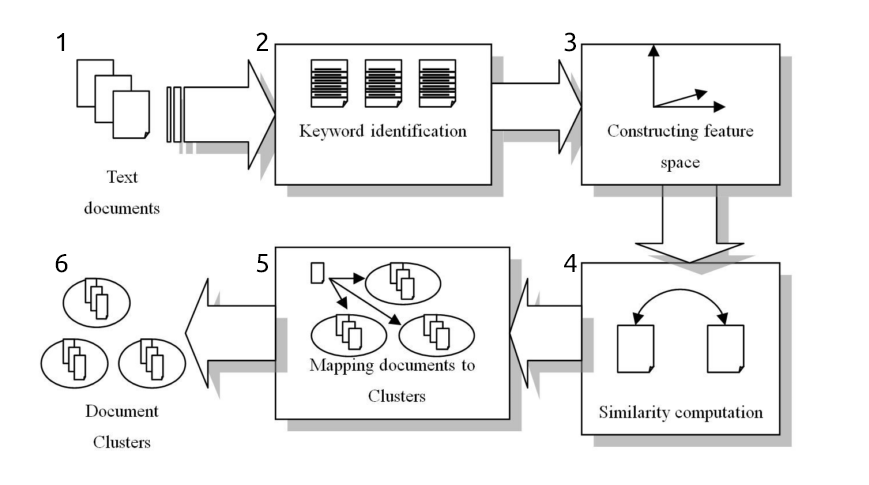
\includegraphics[width=12cm]{images/1_Text_Clustering_Main_Framwork.png}
  \end{center}
  \caption{ Text Clustering Main Framework from~\citet{Dozono2012} }
  \label{fig:1_Text_Clustering_Main_Framwork}
\end{figure}
In the first, step a data set must be provided in order to cluster the documents. 
The second step is where non relevant words are removed from the documents, which greatly improves clustering quality~\cite{Kang2003}. Another way to extract keywords is to differentiate text features by analyzing the document corpora. For example if the dataset is composed from HTML or XML documents it is possible to identify more relevant features due to the characteristics of the document syntaxe.
The fourth step is characterized by converting the keywords of each document into vectors, the most common model used for this task is VSM (Vector Space Model). In VSM, each vector dimension means one detected keyword and each document is represented by the vector of keywords in the feature space. This process an is described in Figure ~\ref{fig:2_svm}.

\begin{figure}
  \begin{center}
    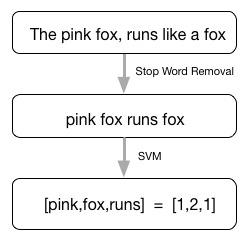
\includegraphics[width=5cm]{images/2_svm.jpg}
  \end{center}
  \caption{ Stop word removal and transformation to Vector Space Model }
  \label{fig:2_svm}
\end{figure}


There many clustering algorithms. K-means works by randomly selecting k documents as the cluster centroids, then assigning each document to the nearest centroid, and finally recalculate the centroid with new added documents. 

\section{The Self-Organizing Map} 
\label{sec:the_self_organizing_map}

\ac{SOM} is a two layer, recurrent \ac{ANN} that has the desired property of topology preservation which mimics the way the cortex of highly developed animals brains work. \ac{SOM} allows cluster visualization of multi-dimensional data, like methods such as \ac{MDS} by \citet{KruskalWish1978} and \ac{PCA} by \citet[]{Hotelling_1933} .  

As \citet{Bacao2005} describes, the basic idea behind SOM is to map the data patterns into an n-dimensional grid of neurons or units. That grid is also know as the output space, as opposed to the initial space also called input space, where the input patterns reside. Both spaces can be seen in Figure~\ref{fig:5_neighbours_converge}.

SOMs work similar to the way that is thought that the human brain works. By having a set of neurons that through learning experience specialize in the identification of certain types of patterns. These neurons are responsible for categorizing the input patterns for which they are responsible to identify. Nearby neurons will be organized by similarity which will cause that similar patterns will activate similar areas of the SOM.
With a topology preserving mapping, SOM organizes the information spatially where similar concepts are mapped to adjacent areas. The topology is preserved in a sense that, as far as possible, neighborhoods are preserved through the mapping process.
Neurons are displayed in an N dimensional grid, generally rectangular, but other structures are possible, such as hexagonal or octagonal.  The grid of neurons, also called output space, can be divided in neighborhoods, where neurons responsible for the same kind of input reside.
In SOM, neurons will have the same amount of coefficients as the input patterns and can be represented as vectors through the VSM model described earlier in Section ~\ref{sub:clustering}.

Before describing the algorithm it is important to define two key aspects of the SOM, the learning rate and quantization error. The learning rate is a function that will be decreased in order to converge to zero, it will be applied to winning neurons and their neighbors in order for them to move toward the corresponding input pattern. Quantization Error is the distance between a given input pattern and the associated winning neuron, it describes how well neurons represent the input pattern. The radius of the neighborhood around the winner neuron is particularly relevant to the topology of the SOM, deeply affecting the unfolding of the output space as stated by \citep{Bacao2005}.
\par

% Self Organizing Map algorithm in latex, needs package algorithm2e
\begin{figure}[h]
  \begin{algorithm}[H]
    \label{alg:som}
    \DontPrintSemicolon
    \KwData{Input patterns $X = \{  \overrightarrow{x_1}$,\dots,$\overrightarrow{x_N}$ \}, number of iterations $t_{\textrm{$max$}}$,  neighborhood function $\sigma(t)$, learning rate  $\epsilon(t)$ }
    \KwResult{Trainned map and clustered input patterns}
    Randomly initialize neurons, $w_i \in \mathbb{R}^{D}, \forall i $ \;
    \For{ $t = 1 \; to \; t_{\textrm{$max$}}$ }{
      Randomly draw an input pattern, $ \overrightarrow{x_d} $  \;
      \nl\label{som:one}$p =  \arg{ min_i \{ \|  \overrightarrow{x_d} - \overrightarrow{w_i} \|  \}}  $  \;
      \nl\label{som:two}$\overrightarrow{w_i} = \overrightarrow{w_i} + \epsilon(t) \cdot h_{ip}(t) \cdot ( \overrightarrow{x_d} - \overrightarrow{w_i} ),  \forall{i}$ \;
      \nl\label{som:three}$\sigma(t) = \sigma_0( \sigma_f / \sigma_0 )^{t/t_{max}}$  \;
      \nl\label{som:four}$\epsilon(t) = \epsilon_0( \epsilon_f / \epsilon_0 )^{t/t_{max}}$ \;  
      \nl\label{som:fifth}$ t \leftarrow t + 1$}
      \caption{Self-Organizing Map \cite[]{Kohonen1990} }
  \end{algorithm}
\end{figure}

The learning phase is characterized by the Algorithm~\ref{alg:som}, which works the following way:
\begin{itemize}
  \item \textbf{Line 1:} The neuron closer to the input pattern is selected. The Euclidean distance (Eq.~\ref{eq:eucl_dist}) is generally used.
    \begin{equation}
  \label{eq:eucl_dist}
  Dist=\sqrt{\sum_{i=0}^{i=n}( V_i-W_i)^2}
\end{equation} 

  \item \textbf{Line~\ref{som:two}:} the winning neuron $(p)$ previously selected on line 1 is updated, in order to better represent the input pattern --- this process is represented on Figure~\ref{fig:4_wining_neuron_converge}. Also, all other neurons inside a specific radius will also be updated --- this process is described in Figure~\ref{fig:5_neighbours_converge}. Each neuron is updated with a different rate of influence determined by how far away it is from the winning neuron, which is defined by the neighborhood influence function $h_ip(t)$. A Gaussian (Eq.~\ref{eq:gaussian}) is often used. 
    \begin{equation}
  \label{eq:gaussian}
  h_{ip}(t)=\exp{-\frac{|\overrightarrow{a_i}-\overrightarrow{a_p}|^2}{\sigma^2(t)}}
\end{equation} 

  \item \textbf{Line~\ref{som:three}:} the size of the radius is updated.
  \item \textbf{Line~\ref{som:four}:} the learning rate is updated.
  \item \textbf{Line~\ref{som:fifth}:} the number of iterations is incremented.
\end{itemize}
 
In order for the algorithm to converge, the learning rate and the radius of the neighborhood need to decrease at a given rate. This process can be seen on line \ref{som:three} and \ref{som:four}, respectively .
%Generally exponential decay is used.


The learning phase is characterized by the training algorithm~\ref{alg:som}, which works the following way:
\begin{itemize}
  \item Neurons can be initialized randomly or it is possible to select a specific initialization.
  \item Given an input pattern, calculate the distance between the input pattern and every neuron on the network. The euclidian distance~\ref{eq:eucl_dist} is generally used.
  \item The winning neuron will be the closest neuron to the input pattern.
  \item The neuron will move towards the data pattern at a given learning rate, in order to improve his representation as can be seen in Figure~\ref{fig:4_wining_neuron_converge}.
  \item Neighbor neurons will also improve their representation in order to keep the network progressively organized as can be seen in Figure~\ref{fig:5_neighbours_converge}.
\end{itemize}

\begin{equation}
  \label{eq:eucl_dist}
  Dist=\sqrt{\sum_{i=0}^{i=n}( V_i-W_i)^2}
\end{equation} 


\begin{figure}
  \begin{center}
    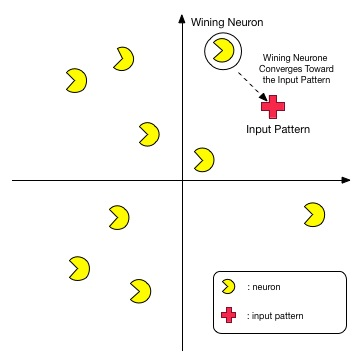
\includegraphics[width=5cm]{images/4_wining_neuron_converge.jpg}
  \end{center}
  \caption{ Winning neuron converging at learning rate }
  \label{fig:4_wining_neuron_converge}
\end{figure}

\begin{figure}
  \begin{center}
    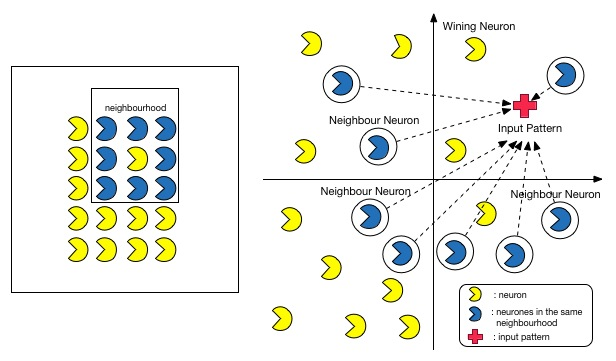
\includegraphics[width=12cm]{images/5_neighbours_converge.jpg}
  \end{center}
  \caption{ On the left the output space neighbor, on the right the neighbors of the winning neuron converging }
  \label{fig:5_neighbours_converge}
\end{figure}

In order for the algorithm to converge, the learning rate and the radius of the neighbourhood need to decrease at a given rate. Generally the exponential decay~\ref{eq:exp_decay} is a good function to decrease both \ac{SOM} characteristics between desired values.
The prediction phase starts after convergence. On the prediction phase new input patterns can be quickly assigned to the SOM, without need to apply the learning rate to the winning neuron and his neighbors. Thus it very easy and fast to classify new data now.

\begin{equation}
  \label{eq:exp_decay}
  \frac{dN}{dT}=-\lambda N
\end{equation} 



In order to visually interpret the result of the SOM U-matrices may be used as stated by ~\citep{Bacao2005}. The U-matrix is a representation of the SOM in which distances, in the input space between neurons is represented using a gray scale.

The advantages of using SOM is data noise immunity, easy to visualize the data, and parallel processing~\cite{Liu2012b}.
 
